\documentclass[12pt]{beamer}
%\documentclass[20pt,handout]{beamer}
\usetheme{Darmstadt}
\usepackage{graphicx}
\usepackage[german]{babel}
\usepackage[T1]{fontenc}
\usepackage[utf8]{inputenc}
\usepackage{tikz}
\setbeamertemplate{footline}[frame number]

\newcommand{\cc}[1]{\includegraphics[height=4mm]{img/#1.png}}
\usepackage{ifthen}
\newcommand{\license}[2][]{\\#2\ifthenelse{\equal{#1}{}}{}{\\\scriptsize\url{#1}}}
\usepackage{textcomp}

\pgfdeclareimage[height=.6cm]{c3d2logo}{./img/c3d2.pdf} 


\pgfdeclarelayer{foreground}
\pgfsetlayers{main,foreground}
\logo{\pgfputat{\pgfxy(-1,0)}{\pgfbox[center,base]{\pgfuseimage{c3d2logo}}}}


\title{Soziale Netzwerke}
\author{\small Marius Melzer \& Paul Schwanse\\\large Chaos Computer Club Dresden}
\date{21.03.2013}

\begin{document}
\maketitle

\section{Einleitung}
\subsection{}

\begin{frame}
  \frametitle{Wer sind wir?}
  \begin{figure}
    
\includegraphics[height=0.7\textheight]{img/fingerabdruck.jpg}
  \end{figure}
\end{frame}

\begin{frame}
  \frametitle{Wer sind wir?}
  \begin{figure}
    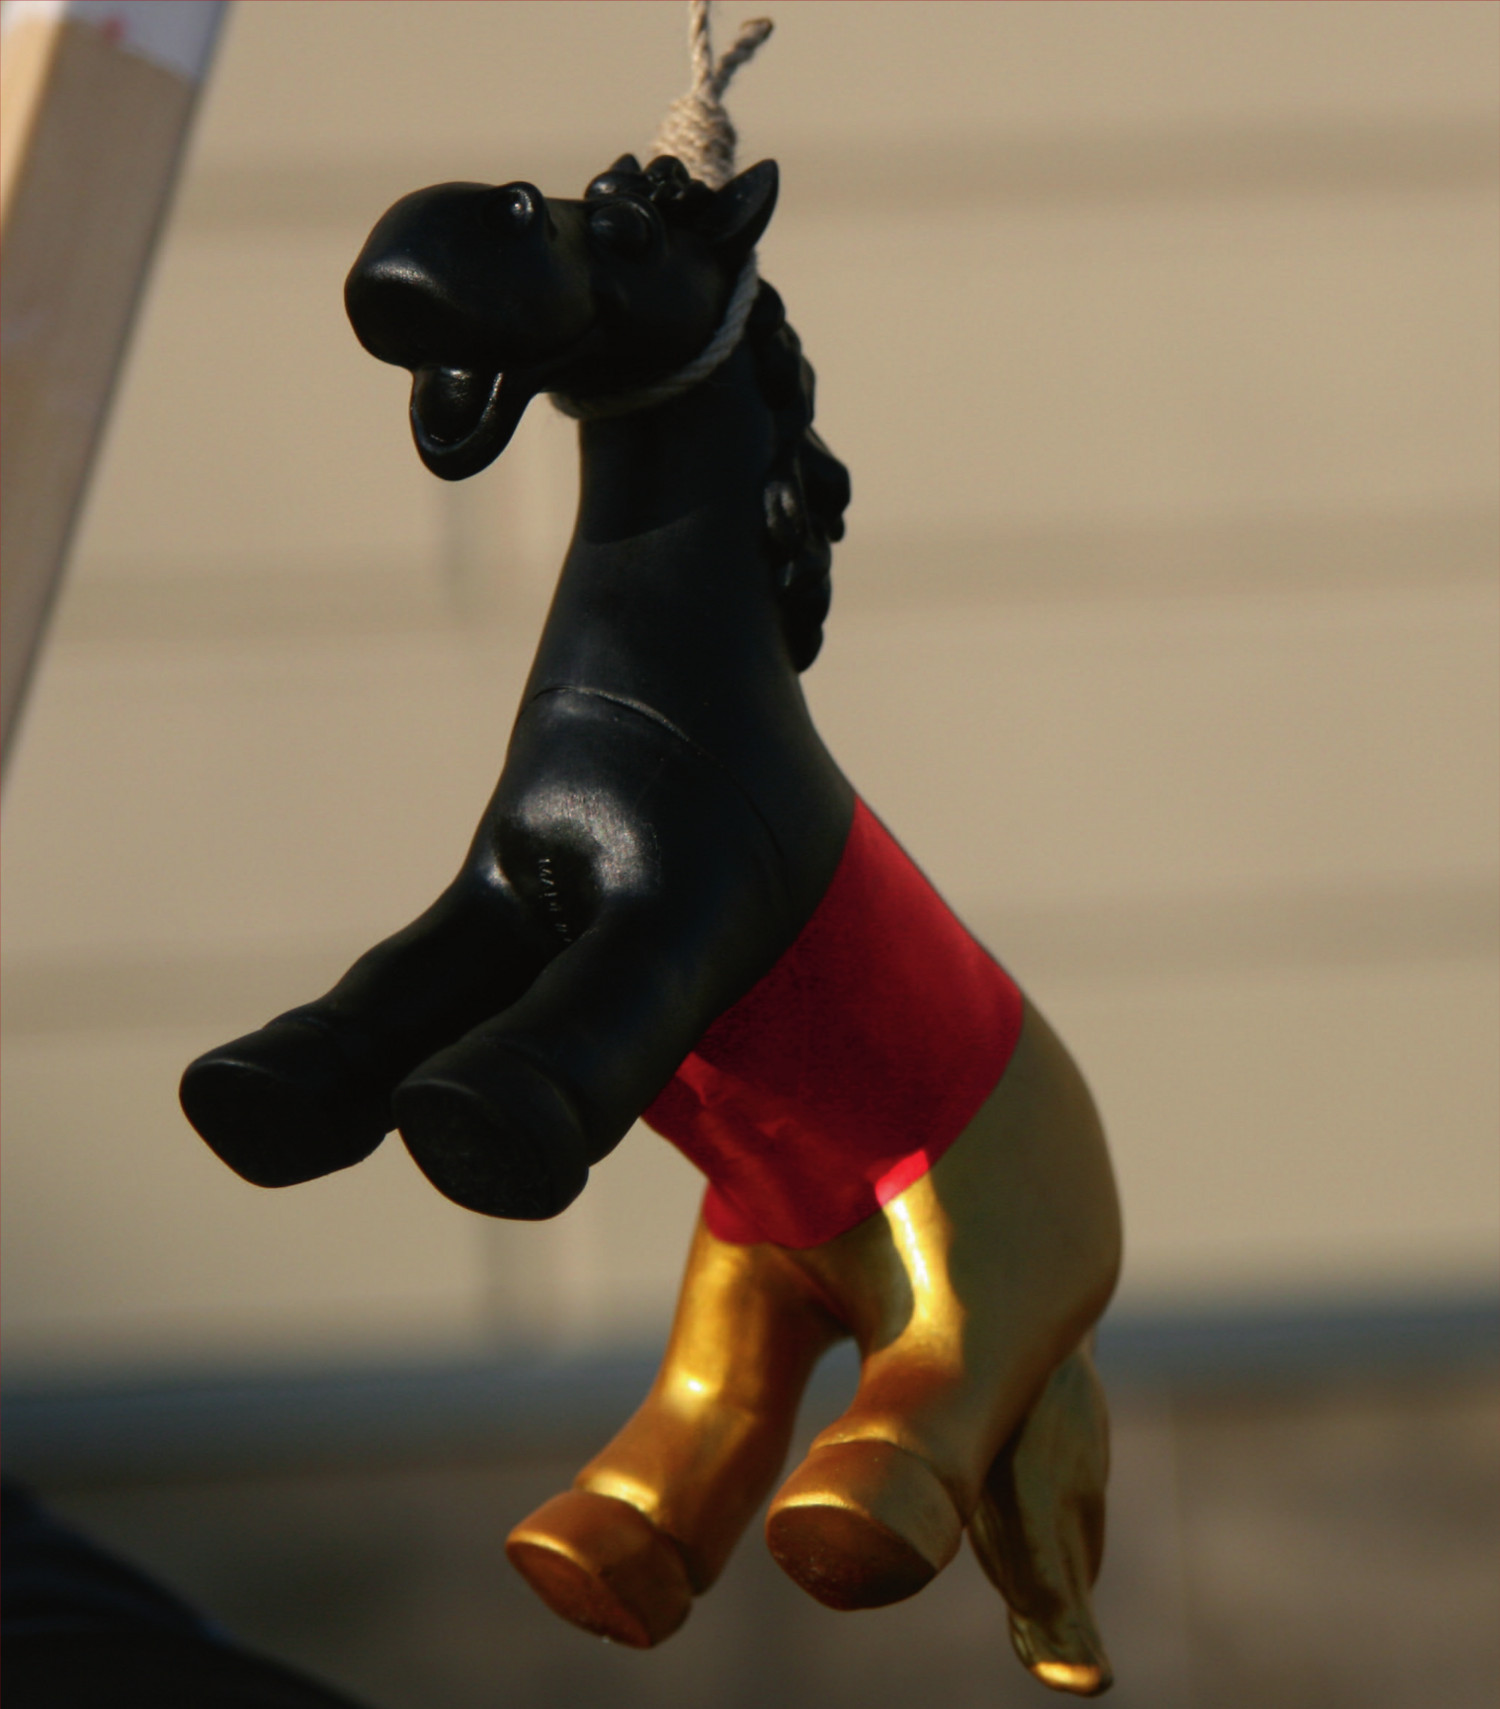
\includegraphics[height=0.7\textheight]{img/trojaner.jpg}
  \end{figure}
\end{frame}

\begin{frame}
    \frametitle{Wer sind wir?}
    \begin{itemize}
      \item<1-> Chaos Computer Club Dresden (\url{http://c3d2.de})
          \note{}
      \item<2-> Datenspuren: 6. und 7. September 2013 \url{http://datenspuren.de}
      \item<3-> Podcasts (\url{http://pentamedia.de})
      \item<4-> Chaos macht Schule
    \end{itemize}
\end{frame}

\end{document}
